\documentclass[jou,11pt]{apa6}
\usepackage[utf8]{inputenc}
\usepackage[table]{xcolor}% http://ctan.org/pkg/xcolor
\usepackage[english]{babel}
\usepackage[natbibapa]{apacite}
\usepackage{graphicx}
\usepackage{enumitem}
\usepackage{tabularx}
\usepackage{booktabs}
\usepackage{setspace}
\PassOptionsToPackage{hyphens}{url}

%\let\OldMaketitle\maketitle
%\let\OldNewpage\newpage
%\renewcommand\maketitle{%
%   \renewcommand\newpage{\let\newpage\OldNewpage}% <----- Eliminate the effect of first \newpage
%   \OldMaketitle%
%}
\renewcommand{\doiprefix}{}
\newcommand{\doi}[1]{https://doi.org/#1}


%http://www.chikrii.com/products/tex2word/
\title{The Validity of Sentiment Analysis:\par Comparing Manual Annotation, Crowd-Coding, Dictionary Approaches, and Machine Learning Algorithms}
\shorttitle{The Validity of Sentiment Analysis}

\twoauthors{Wouter van Atteveldt, Mariken A.C.G. van der Velden}{Mark Boukes}
\twoaffiliations{Communication Science, Vrije Universiteit Amsterdam}{Amsterdam School of Communication Research}

\abstract{Sentiment is central to many studies of communication science, from negativity and polarization in political communication to analyzing product reviews and social media comments in other sub-fields. 
This study provides an exhaustive comparison of sentiment analysis methods, using a 
validation set of Dutch economic headlines
to compare the performance of manual annotation, crowd coding, numerous 
dictionaries and machine learning using both traditional and deep learning algorithms. 
The three main conclusions of this article are that: 
(1) The best performance is still attained with trained human or crowd coding;
(2) None of the used dictionaries come close to acceptable levels of validity; and 
(3) machine learning, especially deep learning, substantially outperforms dictionary-based methods but falls short of human performance.
From these findings, we stress the importance of always validating automatic text analysis 
methods before usage.
Moreover, we provide a recommended step-by-step approach for (automated) text analysis projects to ensure both efficiency and validity. 
}
\keywords{Sentiment Analysis, Manual Annotation, Automated Approaches, Measurement Validity, Evaluation}

\authornote{Accepted for publication in Computational Methods and Measures, details will follow}

\begin{document}

% APA6 seems to want indented paragraphs, but for some reasons the apa6 class does not?
%\setlength{\parindent}{4em}
 
\maketitle

% JoC wants level-2 headings since they see the title as the level-1 heading.
% Add an empty section here so we can use subsections in the rest. 
% Comment out for jou mode, add for man mode
%\section{}

\noindent \emph{Sentiment} (or tone) of communication is a central topic for scholars of communication \citep{lengauer2012negativity}. 
Sentiment has been studied in news coverage of politicians  \citep{hopmann2011incumbency,dunaway2015objectivity,vargo2014network}, news coverage of political elections \citep{kleinnijenhuis2019combined,kleinnijenhuis2007test,mccombes2000setting},
political campaigns \citep{cho2013campaign,shah2007campaign,haselmayer2019negative,Nai2019,Ridout2011}, political referendums \citep{elenbaas2008effects}, political debates \citep{nagel2012there,connaughton2004invitations,hopmann2011incumbency}, and to analyze the rhetoric of political elites in parliament and manifesto's \citep{Rhodes2019,Rheault2016,Kosmidis2018} -- to name a few topics in the last two decades. 
Beyond the domain of politics, a wide variety of communication scholars used sentiment to study objects, such as the quality of mediated inter-group contact \citep{wojcieszak2016saw}, the hostile media effect \citep{shin2017partisan}, news coverage of wars \citep{aday2010chasing}, news coverage of Asia in Asian and Western TV stations \citep{natarajan2003asian}, coverage about companies \citep{jonkman2020buffering}, media violence and aggression \citep{martins2013content}, health news coverage \citep{kim2015attracting}, the content of news websites \citep{valenzuela2017behavioral} and the user-comments under their articles \citep{muddiman2017news}, gender differences in news reporting  \citep{rodgers2003socialization}, news frames on biotechnology \citep{matthes2008content}, or criticisms of news media \citep{domke1999politics}.

While omnipresent as a concept, measuring sentiment -- or any of the often co-occurring concepts, such as emotionality, negativity, polarity, subjectivity, tone, or valence -- is not straightforward. 
Sentiment is generally expressed with ambiguous and creative language \citep{pang08,wiebe04,liu12}.
In addition, sentiment analysis in the social sciences suffers from a lack of agreed-upon conceptualization and operationalization \citep{lengauer2012negativity,kleinnijenhuis2008negativity}. 

Computational approaches to sentiment analysis have the potential to remedy the problems of scalability and replicability inherent in manual coding 
\citep[For overviews, see for example][]{vanatteveldt2019studying, welbers17, boumans16}.
%To remedy the costs and logistic difficulties involved with human annotation, scholars have increasingly relied upon automated forms of text analysis 
% The ``text-as-data revolution'' \citep{grimmer13} has blessed us with many easy available new data sources to test old and new research questions.
% The fast-growing computational text community has made it possible to use these newly available data sets -- a prime example hereof is the R-package \emph{Quanteda} \citep{quanteda}. 
While these methods can be very cost-efficient, their application is not without pitfalls \citep{grimmer13,wilkerson2017large,margolin2019computational,hilbert2019computational,atteveldt2018cmm}.
Off-the-shelf dictionaries are developed for, and typically validated on, a specific task and domain, and often do not perform well on other tasks. 
For example, \citet{young12} found that different dictionaries for measuring sentiment ``show stunningly little overlap'' (p.211)
and do not correlate well with each other or with expert annotations. 
Similarly, machine learning models that are optimized for a certain task (such as distinguishing positive film reviews from negative ones) can give misleading results for social science research by identifying spurious patterns in the data that was used to train these algorithms \citep{thelwall2012sentiment}.
Nevertheless, the current proliferation of available dictionaries and other off-the-shelf tools tends to overshadow the low measurement validity \citep{gonzalez15, soroka15},
and in many cases these tools are not validated before being used on new tasks. 
On top of these challenges, (semi-)automated tools for non-English languages are rare, hampering comparative research of communication \citep{haselmayer2017sentiment}. 

This paper's contribution lies in demonstrating which, if any, of the sentiment analysis methods actually work well for determining the tone of media coverage.
We use a triple-coded gold standard validation set to compare different manual and automatic approaches to sentiment analysis of Dutch economic news headlines.
Using a Dutch-language case study gives an impression of the state of the art in non-English language tools 
as well as allowing us to test the efficacy of machine translation for comparative research.
Moreover, we presume that journalistic descriptions of whether the economy is doing well or not are relatively factual and unambiguous. 
Therefore, the economy seems to be an `easy' test for automated methods compared to many aspects of political news,
where opinions and sentiment are often expressed in more nuanced or creative ways. 

%Using only the headlines of text also simplifies the problem since 
Headlines are often relatively simple and explicit compared to the more nuanced arguments made in the article body. 
%Moreover, it 
Thereby, focusing only on headlines avoids the issue of articles citing multiple sources that can each express a different sentiment, which makes it difficult to judge the `overall' sentiment of an article.
%On the other hand, 
Nevertheless, the limited amount of words in a headline could put automatic methods at a disadvantage since it is less likely that any given dictionary or machine learning model will contain a matching word.
The sentiment of headlines, however, is interesting in its own right as the headline is the first (and sometimes the only) part of an article that people read, and headlines shape the context in which people read the article. 
In social science research, headlines are seen as an important framing device \citep[e.g.][]{tankard01,liu19}, 
a signal of news values \citep[e.g.][]{ng20} and as an important predictor of effects on polarization, political attitudes, and consumer confidence \citep[e.g.][]{munger20,narayan17,blood95}.
Moreover, many other forms of communication that are studied in our field (and with automated content analysis), such as tweets, chat messages, and online comments, are also relatively short.
Thus, evaluating methods that determine sentiment of headlines is a relevant task for communication science.
In addition, it is a suitable case for sentiment analysis in general,
even though results might differ for other forms of communication such as full articles.


%We fully agree that headlines are not the same thing as the full article, and it’s fully possible that a headline has a strong sentiment while the article itself is more nuanced and balanced. The sentiment of headlines, however, is interesting in its own right as the headline is the first (and sometimes the only) part of an article that people read and is an important context in which they read it. In communication research, headlines are seen as an important framing device (e.g. Tankard 2001, De Vreese 2005, Liu et al 2019) a predictor of whether people are likely to read the full article (e.g. Lagerwerf 2020, Ng & Zao 2019) and as predictor of media effects on polarization (e.g. Munger et al., 2020), market prices (e.g. Narayan & Narayan 2019), and political attitudes (e.g. Blood & Philips, 1995). Moreover, besides headlines other short texts such as tweets, chat messages, and online comments are also relatively short but important forms of communication that are often studied in our field. 


For this study, we used the existing manual annotations presented in \citet{boukes2019}.
Besides comparing the gold standard to these manual codings and to crowd coding data that were collected specifically for this article, 
we used the manual codings as training data for classical and `deep learning' machine learning models.
%In this paper, we evaluate many different approaches to measure sentiment in text with methods that go beyond off-the-shelf Dutch dictionary tools. 
Finally, we apply many of the different dictionaries that have recently become available,
including English-language dictionaries using machine translation of the headlines \citep[e.g. as suggested by][]{devries2018} and a dictionary specifically customized to the domain of interest \citep[suggested by][]{muddiman2019}. 
Thereby, our paper presents a comprehensive review of existing methods to measure sentiment.
We apply an open science, open materials approach. 
All our analytical code, data, and results are published in the online compendium for this paper.%
%\footnote{For review, an anonymous version of this compendium is available here: \url{https://anonymous.4open.science/r/475de8a9-6796-4538-95bc-94182a2e5557/}}
\footnote{\url{https://github.com/vanatteveldt/ecosent}}

Generally, results from this case study do not warrant optimism regarding the possibilities of automatic sentiment analysis, especially dictionary based analyses. 
In line with e.g. \citet{soroka15} and \citet{boukes2019}, we find that off-the-shelf dictionaries perform poorly on this task.
Machine learning approaches, especially deep learning, performs considerably better than the off-the-shelf sentiment analysis tools, 
but still do not reach the level of validity generally required for text analysis methods. 
On a more positive note, the results of crowd coding can compete with the quality delivered by trained coders, providing a cheaper and especially more transparent and replicable alternative to expensive student coders. 
The main take-home message is, however, that a human eye is still required to guarantee the validity of measuring sentiment in content analysis.
As detailed in the step-by-step process given at the end of this article, we strongly recommend that every automatic text analysis project should start with coding a validation set. 


\section{Existing Methods of Sentiment Analysis}

\noindent Traditionally, sentiment is measured using manual annotators and a codebook \citep[for examples, see][]{kleinnijenhuis2019combined,kleinnijenhuis2007test,meijer2006issue,cho2013campaign,shah2007campaign,aday2010chasing,elenbaas2008effects,natarajan2003asian,mccombes2000setting,martins2013content,nagel2012there,rodgers2003socialization,muddiman2017news,dunaway2015objectivity}. %or all of the intro citations?
Manual coding is expensive, however, and even when using extensive training programs high levels of reliability are not always achieved \citep{weber18}.
%This not only complicates measuring sentiment: Extensive training, in combination with uncertain data quality, makes measuring sentiment even more expensive.
%To avoid the high costs of manual coding, scholars have turned to the `wisdom of the crowd’ and used crowd-coding as a compelling solution for the huge volumes of available texts 

One possible solution is to use crowd coding platforms instead of traditional expert (or undergrad) coders \citep{benoit16,haselmayer2017sentiment,lind2017content}.
Sentiment analysis, in particular, can be relatively easily reduced to simple questions suitable for crowd coding.
In addition, the lower costs of crowd coding allow for each document to be coded by multiple coders.
This not only increases reliability, but also gives an indication of the ambiguity of sentiment.
Finally, the crowd only sees the material as presented in the crowd coding platform, which can be easily shared between researchers.
This means that crowd coding is more transparent and replicable than traditional manual coding.

Another option is to use automatic sentiment analysis methods: 
Using a computer program to classify each document as being positive, neutral, or negative
\citep[for overviews of these methods, see][]{grimmer13,wilkerson2017large,welbers17,vanatteveldt2019studying,boumans16,hopkins2010method, nunez2016automated}. 
There are broadly two types of methods that can be used for this: dictionaries and supervised machine learning. 

%As a solution, scholars turned to new common practice where computers `do the work' instead of costly human annotators. 
%When using computers -- or better to say \emph{automated} or \emph{computational} methods -- for text analysis, scholars `ask the computer' for \emph{classification} 
%That is, to organize texts into a set of categories. 
%Sometimes researchers know the categories beforehand -- for instance, positive and negative utterances -- other times they do not. 
%In the case of sentiment, or any of its synonyms, the categories are known. 
%One is interested in the occurrence of positive utterances relative to the occurrence of negative ones for the object of study.

One could (naively) think that measuring sentiment using a dictionary should be easy:
Make a long list of positive and negative words and count how many words of each category occur.
Indeed, in the last decade we have seen a proliferation of available \emph{off-the-shelf} dictionaries for sentiment analysis \citep{gonzalez15, soroka15}.
Studies within computational linguistics, however, suggest that coming up with the right set of keywords might be less trivial than one initially thinks \citep[for an overview, see][]{pang08}. 
Applying one or another dictionary to investigate a specific research question could lead to widely divergent conclusions \citep{boukes2019,young12,gonzalez15,soroka15}.

In general, it turns out that the validity of sentiment analysis highly depends on the domain, genre and language to which it is applied \citep{gonzalez15,soroka15,pang08,thelwall2012sentiment}.
Therefore, scholars have started to apply (supervised) machine learning methods to classify texts. % -- or video's and images.
In contrast to the off-the-shelf dictionaries, machine learning can account for the peculiarities of the texts under study.
In machine learning, rather than having the researcher specify this link explicitly using a dictionary,
the computer uses manually coded \emph{training data} to learn the link between input features (e.g. words as independent variables) and the desired output label (e.g. sentiment as dependent variable).
Technically, a machine learning algorithm is used to create a statistical model based on the training data which is then used to 
predict the sentiment of unlabeled texts.
%That is, a sentence like ``The econonomy has never been better'' has the label `positive', while a sentence like ``The economy took a big hit'' is labeled negative.
Machine learning generally outperforms dictionary-based methods, and most state-of-the-art sentiment analysis systems developed in computational linguistics are now based on machine learning \citep{semeval}. 
These models generally have a very high number of parameters to be estimated, for example a score for every unique word in the training data.
Since this can easily lead to overfitting of the model, 
its performance should always be judged on separate validation data (out of sample prediction).

Initially, most machine learning applications used word frequencies -- also called `bag-of-words' -- as input features.
This approach ignores all aspects of word order and grammar. 
More recently, so-called `deep learning' models have been developed that use neural networks with many hidden layers to overcome this limitation \citep{goldberg17}. 
This is generally used in combination with \emph{word embedding models} \citep{mikolov13distributed, rudkowsky2018more}. 
These models used very large quantities of unlabeled texts (i.e. without manual codings) 
to learn the overall meaning of a word.
This reduces the number of distinct input features and allows words that were not present in the initial data to be captured in the model. 

Each of the methods surveyed here has its own advantages and disadvantages.
Although machine learning methods generally outperform dictionaries in state-of-the-art systems, 
their performance strongly depends on the availability of sufficient training material.
Dictionaries are more transparent and easier to apply.
All automated methods, however, will decrease in performance when applied to a task or domain
that is different from the one it was developed for. 
This makes it difficult to estimate beforehand which method will be the most effective or what its performance will be.
The difficulty of ex-ante estimation stresses the importance of validating each method for its specific task. 

%This means the computer can also take word context or word combinations into account.

%A variety of choices could be made when applying SML.
%For examply which \emph{algorithm} should I apply? Or who is attaching the labels to texts that the computers in turn have to learn the patterns of?
%To address the first question, very broadly speaking, one could distinguish \emph{classical} machine learning from \emph{deep learning}.
%The first one is quite similar to training a regular statistical model, with the word counts as input variables and the sentiment (positive, neutral, negative) as a nominal outcome variable. 
%Deep learning is a non-scientific term to refer to a class of models that have been developed relatively recently.
%These models are called `deep' learning because they generally consist of a neural network with multiple `hidden' (latent) layers, that take individual words as input rather than aggregated word counts. 
%To answer the second question, the `gold standard’ to compare the outcomes of the automated approaches against, is typically created by a manual content analysis, following established best practices for safeguarding reliability \citep{balke2014agents,krippendorff12,taboada11}. 
%To avoid the high costs of manual coding, scholars have turned to the `wisdom of the crowd’ and used crowd-coding as a compelling solution for the huge volumes of available texts \citep{benoit16,haselmayer2017sentiment,lind2017content}.


\section{Data and Methods}

\noindent By comparing various methods of sentiment analysis, 
this paper aims to help researchers choose the best method for approaching a sentiment analysis project.
The starting point of this analysis are the data reported in \cite{boukes2019}.
%To compare the various methods of sentiment analysis with the aim of giving researchers a recommendation how to approach the measurement of sentiment analysis, .
These authors collected news from a total of ten newspapers and five websites using an extensive search string that covers a wide variety of economic and financial issues published between February 1 and July 7, 2015. It included three quality newspapers (\textit{NRC Handelsblad, Trouw, de Volkskrant}), a financial newspaper (\textit{Financieel Dagblad}), three popular newspapers (\textit{Algemeen Dagblad, Metro, De Telegraaf}) and three regional outlets (\textit{Dagblad van het Noorden, de Gelderlander, Noordhollands Dagblad}). 
For the automated text analyses, all headlines were preprocessed by lemmatizing them using the Dutch lemmatizer Frog \citep{frog}.
In short, lemmatizing means that we reduce a verb like ``dacht'' (thought) to its lemma ``denken'' (think). 
%Newspapers items were retrieved via LexisNexis and stored in the Amsterdam Content Analysis Toolkit (AMCAT) \citep{vanatteveldt2014}. The items of the news websites were retrieved from the Infrastructure for Content Analysis-tool (INCA) \citep{trilling2018}. 

\paragraph{Gold Standard}
To guarantee the quality of our comparisons, we have created a gold standard against which we evaluate the existing methods by manually annotating a selection of the headlines from the manually annotated data of \cite{boukes2019}.
We randomly selected headlines that were annotated multiple times and that were annotated as being about the economy. 
\citet[p.240]{krippendorff12} recommends at least 143 documents for determining intercoder reliability for this case ($P_c =.33;\alpha\geq.8;sig.\leq.005$), but to be conservative we decided to use 300 headlines.
%This choice allowed us to focus on comparing sentiment analysis methods instead of comparing topic and sentiment jointly.
These headlines were annotated by the three authors using the instructions from the original article.
The initial inter-coder agreement of this coding was Krippendorff's $\alpha=0.75$,
with agreement between coder pairs ranging from 0.75 to 0.82, which reflects the subjectivity of the task at hand. 
All disagreements were then discussed between the authors and resolved where possible.
In most cases, these disagreements were caused by simple clerical errors or by a misinterpretation of the sentence or coding rules. 
Eleven headlines were removed after discussion as they were deemed to be inherently ambiguous (i.e., not ideal for a gold standard),
If anything, removing the hardest headlines should make the task slightly easier for the different forms of automatic sentiment analysis. 

\paragraph{Manual Coding}
As reported in \citet{boukes2019}, the sentiment of newspaper and website headlines was manually annotated by a team of 22 student coders. 
The coders were trained by means of two training sessions of three hours, and three homework assignments. 
In addition, they could send their questions or doubts by e-mail and receive almost immediate feedback. 

To verify whether articles really dealt with economic news, the first question in the code-book was whether the headline or first paragraph of the item referred to the economy, economic developments or an economic topic (e.g., inflation, unemployment, interest rates, or the housing market). 
Subsequently, coders were asked to evaluate the sentiment of a headline with regards to the economy on a three point-scale: (-1) negative; (0) neutral, ambiguous, or mixed; and (+1) positive. 
Coders were explicitly instructed to only evaluate the headline and to not consider any information that they already had seen from the full text. 
Inter-coder reliability was assessed on sample of 148 randomly selected news items that were analyzed by at least three of the coders; on average this were 5.63 coders. This sentiment measurement proved to have a satisfactory inter-coder reliability (Krippendorff's $\alpha$ = .80).

\paragraph{Crowd Coding}
The headlines from the gold standard were all coded by five crowd coders using the Figure~8 platform.\footnote{\url{http://figure-eight.com}, formerly CrowdFlower} 
Coders received short instructions with a limited amount of examples (see online appendix for the task definition).
Besides these 300 sentences, 70 (relatively straightforward) test sentences were included for which we provided the correct answer.
These were used first in an initial quiz to ensure coders understood the instructions, and after that one test question was included in every page of five target sentences to ensure that coders remained concentrated during the task. Coders that missed test questions were informed of this, and coders missing more than 70\% of test questions were excluded. 


\paragraph{Sentiment Dictionaries} 
In this paper, we partly replicate the dictionaries used in \cite{boukes2019} and add specific dictionaries for \textit{hope} and \textit{fear} in the economic context.
Specifically, we applied the Dutch ANEW \citep{anew}, Pattern \citep{pattern} and Polyglot \citep{polyglot} dictionaries 
using the Python code published with that paper. 
In addition, we used the R package Quanteda \citep{quanteda} to add 
(a) the dictionary developed by \cite{damstra2018} to measure the sentiment of economic news; 
(b) the NRC Emotion Lexicon \citep{mohammad2013} for both measuring positive and negative words as well as trust and fear words; 
and (c) a customized dictionary based on the approach suggested by \cite{muddiman2019}.
%For the latter dictionary, we manually annotated the 300 most frequent words, yielding a dictionary consisting of 32 positive and 38 negative words.
The upper-part of Table \ref{tab:info} displays the number of words per category in the Dutch dictionaries.
For the dictionaries applied using Quanteda (D2, D3, and D4), 
the table also lists the categories that were used for positive and negative words. 
For these dictionaries, a headline was counted as positive if there were more positive than negative words, and similarly for negative.
Headlines without any sentiment words or with equal positive and negative words were treated as neutral. 
%\footnote{The positive category for DamstraBoukes is Hope, the negative one is Fear. For RID, the positive category is Positive Affect, the negative one is Anxiety. For NRC, we first added respectively the positive categories (Positive and Trust) and the negative categories (Negative and Fear), and subsequently used Equation \ref{eq:sentiment}.}}


\paragraph{English Dictionaries using Machine Translation}
The number of Dutch dictionaries available is rather limited. 
There are many more dictionaries for sentiment analysis available in English, 
including also domain-specific dictionaries for sentiment in finance.
Following the suggestion by \cite{devries2018}, we used machine translation to translate the gold standard texts.
For this, we used both Google Translate and DeepL to translate the gold standard texts.%
\footnote{Accessed at \url{https://translate.google.com/} and \url{deepl.com}, respectively. Since DeepL provided slightly better performance, we only report these scores here, but see the online compendium for a full overview. }
This allowed us to make use of the plenitude of English sentiment dictionaries available using the Quanteda R packages \citep{quanteda}:
First, we used the Affective Norms for English Words (AFINN) \citep{afinn}, a publicly available list of English words rated for valence with values between -5 (negative) and +5 (positive). The version implemented in the Quanteda package uses a binary classification. % into 878 positive (valence > 0) and 1,599 negative (valence < 0) features. 
Second, we used the Augmented General Inquirer\footnote{\url{http://www.wjh.harvard.edu/$\sim$inquirer/ homecat.htm}} \textit{Positiv} and \textit{Negativ} dictionary.
Third, we used the dictionary %containing 2,006 positive and 4,783 negative words 
from Hu and Liu \citep{hu2004,liu2005}.
Fourth, we applied the 2014 version of the Loughran and McDonald Sentiment Word Lists \citep{loughran2011}. 
%The categories we used are ``negative'' (2355 features) and ``positive'' (354).
Fifth, we employed the Martindale's Regressive Imagery Dictionary (RID) \citep{martindale1975, martindale1992}.
%The RID consists of about 3,150 words and roots assigned to 29 categories of primary process cognition, 7 categories of secondary process cognition, and 7 categories of emotions, designed by \cite{martindale1975, martindale1992} to measure primordial vs. conceptual thinking.
Sixth, we used the Lexicoder Sentiment Dictionary (LSD) \citep{lexicoder,young12}.
%The dictionary consists of 2,858 ``negative'' sentiment words and 1,709 ``positive'' sentiment words. 
The seventh and eight dictionaries are the NRC Emotion Lexicon, but in English this time, and the translated \cite{damstra2018} dictionary similar to the one applied in Dutch.
The lower-part of Table \ref{tab:info} displays the used categories and number of words per category in the English dictionaries.

\begin{table*}[h!]
  \caption{Information on Off-the-Shelf Dictionaries}\label{tab:info}
\begin{center}\onehalfspacing
\begin{tabularx}{\linewidth}{lXXr}
\toprule
	 \multicolumn{2}{l}{Dictionary} & Category & \# Words \\ 
	 \midrule
	 \multicolumn{3}{l}{\emph{Dutch Dictionaries }}\\
	 & D1: DANEW & (continuous scale) & 4,299 \\
	 & D2: DamstraBoukes & Hope & 30\\
	 & & Fear &  33\\
	 & D3: Muddiman & Positive& 32\\
	 & & Negative & 38\\
	 & D4: NRC: & Positive + Trust & 3,162\\
	 & & Negative + Fear & 4,037 \\
	 & D5: Pattern & Positive ($valence>0$) & 1,554 \\
	 &  & Negative ($valence<0$) & 2,364 \\
	 & D6: Polyglot & Positive & 1,502\\
	 & & Negative & 2,474\\\\
	 \multicolumn{3}{l}{\emph{English Dictionaries }}\\
	 & E1: AFNINN & Positive ($valence>0$)& 878\\
	 & & Negative ($valence<0$) & 1,599 \\
	 & E2: DamstraBoukes & Hope & 30\\
	 & & Fear & 33 \\
	 & E3: GenInq & Positiv & 1,653\\
	 & & Negativ & 2,010\\
	 & E4: HuLiu & Positive&  2,006\\
	 & & Negative & 4,783\\
	 & E5: LoughranMcDonald & Positive& 354\\
	 & & Negative & 2,355 \\
	 & E6: LSD & Positive & 1,709\\
	 & & Negative & 2,858\\
	 & E7: Muddiman & Positive& 32\\
	 &  & Negative & 38\\
	 & E8: NRC & Positive + Trust & 3,543\\
	 & & Negative + Fear &  4800 \\
	 & E9: RID & Positive Affect & 70\\
	 & & Anxiety & 49\\
\bottomrule
\end{tabularx}
\end{center}

\end{table*}

\paragraph{Machine Learning} \label{ML}
This paper uses two types of machine learning: 
`classical' machine learning with a Naive Bayes (NB) and Support Vector Machine (SVM) classifier, and `deep' learning using a Convolutional Neural Network (CNN).
The setup and training procedure for both models are given below.
For all models, we used 6,038 manually coded headlines from \citet{boukes2019} as training data. 
The final models were validated against the 300 headlines gold standard.%
\footnote{
Since the models were trained on the headlines coded by the student coders as reported by \citet{boukes2019},
it is possible that these models would perform better when validated against the student codings rather than against our gold standard data, 
even though we used the same coding procedure. 
To make sure the ML models were not disadvantaged, we also validated the models against the student codings of the gold standard data,
which yielded almost identical results. See the online appendix for these outcomes. }

For the NB and SVM model, we used \emph{scikit-learn} \citep{sklearn} to create a document-term matrix with normalized td-idf weights,
and train and test the model. 
To determine the hyperparameters for the SVM model (regularization parameter and kernel type and coefficient)
we performed a grid search using 5-fold crossvalidation.\footnote{See the online appendix for the grid search procedure and results}
The best performing model was then trained on all training data and tested on the validation set. 
%The choice of machine learning algorithm is determined by the kind of model that fits the data.
%This choice is comparable to choosing between different types of regression models.
%\textbf{Note that SVM is one of many different types of machine learning algorithms, 
%and there are no strong a priori  theoretical considerations for preferring SVM over e.g. Naive Bayes (NB)}. 
%For that reason, we tested different models (and model settings) using cross-validation within the training data. 
%The Support Vector Machine (SVM) algorithm turned out to give the best performance.


%\subsection{Model II:  Convolutional Neural Network}
For the deep learning model, we chose to use a Convolutional Neural Network (CNN), 
which allows for local interactions between word meanings.
That is, scores are computed for windows of adjacent words, so the model can treat word combinations differently from the underlying words. 
Given the relatively small length of newspaper headlines, we decided not to use more complicated models (such as Long-Short Term Memory or LSTM models) that also allow non-local interactions \citep{goldberg17}.
Specifically, we used \emph{keras} with \emph{tensorflow} back-end \citep{tensorflow} to train and test the CNN consisting of the following layers:
\begin{APAenumerate}%[topsep=0pt,itemsep=-1ex,partopsep=1ex,parsep=1ex]
    \item An \emph{embeddings} layer using the Amsterdam Embeddings Model trained on Dutch news \citep{aem}. This layer looks up each word in the input and replaces it by its 320-dimensional embedding vector representing its position in a latent semantic space.
    \item A \emph{convolution} layer that concatenates the embeddings for each 3-word window and transforms them into a lower-dimensional representation using a dense neural layer, effectively allowing for features to be created spanning at most 3 words.
    \item A \emph{max-pooling} layer that maximizes the value for each feature for each document.
    \item A regular \emph{dense network} that predicts the sentiment from the pooled input features. 
\end{APAenumerate}

The architecture above is a relatively standard architecture for document classification. 
However, there are still many choices (hyperparameters) left, from the depth and size of the dense network to the learning rate and loss function. 
Since again there are no strong theoretical grounds to determine these parameters, we conducted a grid search using cross-validation within the training to find the optimal parameter values similar to the procedure for SVM.\footnote{See the online appendix for the grid search procedure and results}
These settings were then used to train a new model on all training data, which was validated on the gold standard data. 




\section{Results} 

%\subsection{Overall Performance of Methods}

\begin{table*}[ht!]
  \caption{Overall Performance of the Tested Sentiment Analysis Approaches}\label{tab:performance}
\footnotesize
\begin{tabularx}{\textwidth}{lXXrrrrrrrr}
\toprule
& & & & & \multicolumn{3}{c}{Positive} & \multicolumn{3}{c}{Negative} \\
\cmidrule(r){6-8}\cmidrule(l){9-11} 
\multicolumn{3}{l}{Method} & Acc. & $\alpha$ & Pr. & Re. & F1& Pr. & Re. & F1 \\
\midrule

\multicolumn{11}{l}{\emph{ Manual Coding }} \\

 & \multicolumn{2}{l}{ Single Coder }& \cellcolor[gray]{0.59} 0.82& \cellcolor[gray]{0.59} 0.82& \cellcolor[gray]{0.56} 0.88& \cellcolor[gray]{0.57} 0.86& \cellcolor[gray]{0.57} 0.87& \cellcolor[gray]{0.58} 0.84& \cellcolor[gray]{0.60} 0.80& \cellcolor[gray]{0.59} 0.82\\

 & \multicolumn{2}{l}{ Vote (3 Coders) }& \cellcolor[gray]{0.56} 0.88& \cellcolor[gray]{0.55} 0.90& \cellcolor[gray]{0.52} 0.97& \cellcolor[gray]{0.54} 0.91& \cellcolor[gray]{0.53} 0.94& \cellcolor[gray]{0.56} 0.87& \cellcolor[gray]{0.58} 0.84& \cellcolor[gray]{0.57} 0.86\\


\multicolumn{11}{l}{\emph{ Crowd-Coding }} \\

 & \multicolumn{2}{l}{ Single Coder }& \cellcolor[gray]{0.64} 0.72& \cellcolor[gray]{0.62} 0.75& \cellcolor[gray]{0.65} 0.69& \cellcolor[gray]{0.58} 0.84& \cellcolor[gray]{0.62} 0.76& \cellcolor[gray]{0.61} 0.78& \cellcolor[gray]{0.61} 0.78& \cellcolor[gray]{0.61} 0.78\\

 & \multicolumn{2}{l}{ Vote (3 Coders) }& \cellcolor[gray]{0.62} 0.77& \cellcolor[gray]{0.60} 0.81& \cellcolor[gray]{0.63} 0.73& \cellcolor[gray]{0.55} 0.89& \cellcolor[gray]{0.60} 0.80& \cellcolor[gray]{0.58} 0.83& \cellcolor[gray]{0.59} 0.81& \cellcolor[gray]{0.59} 0.82\\

 & \multicolumn{2}{l}{ Vote (5 Coders) }& \cellcolor[gray]{0.62} 0.77& \cellcolor[gray]{0.59} 0.81& \cellcolor[gray]{0.63} 0.73& \cellcolor[gray]{0.55} 0.90& \cellcolor[gray]{0.60} 0.81& \cellcolor[gray]{0.58} 0.84& \cellcolor[gray]{0.60} 0.80& \cellcolor[gray]{0.59} 0.82\\


\multicolumn{11}{l}{\emph{ Machine Learning }} \\

 & \multicolumn{2}{l}{ CNN }& \cellcolor[gray]{0.68} 0.63& \cellcolor[gray]{0.75} 0.50& \cellcolor[gray]{0.66} 0.68& \cellcolor[gray]{0.76} 0.49& \cellcolor[gray]{0.72} 0.56& \cellcolor[gray]{0.64} 0.72& \cellcolor[gray]{0.71} 0.57& \cellcolor[gray]{0.68} 0.63\\

 & \multicolumn{2}{l}{ SVM }& \cellcolor[gray]{0.71} 0.58& \cellcolor[gray]{0.79} 0.42& \cellcolor[gray]{0.65} 0.70& \cellcolor[gray]{0.81} 0.38& \cellcolor[gray]{0.75} 0.50& \cellcolor[gray]{0.68} 0.64& \cellcolor[gray]{0.75} 0.49& \cellcolor[gray]{0.72} 0.56\\


\multicolumn{11}{l}{\emph{ Dictionaries }} \\

 & \multicolumn{2}{l}{ DANEW }& \cellcolor[gray]{0.79} 0.42& \cellcolor[gray]{0.95} 0.10& \cellcolor[gray]{0.62} 0.75& \cellcolor[gray]{0.96} 0.08& \cellcolor[gray]{0.93} 0.15& \cellcolor[gray]{0.60} 0.80& \cellcolor[gray]{0.98} 0.04& \cellcolor[gray]{0.96} 0.08\\

 & \multicolumn{2}{l}{ DamstraBoukes }& \cellcolor[gray]{0.80} 0.41& \cellcolor[gray]{0.97} 0.05& \cellcolor[gray]{0.58} 0.83& \cellcolor[gray]{0.97} 0.07& \cellcolor[gray]{0.94} 0.13& \cellcolor[gray]{1.00} 0.00& \cellcolor[gray]{1.00} 0.00& \cellcolor[gray]{1.00} 0.00\\

 & \multicolumn{2}{l}{ Muddiman }& \cellcolor[gray]{0.76} 0.49& \cellcolor[gray]{0.84} 0.31& \cellcolor[gray]{0.74} 0.53& \cellcolor[gray]{0.81} 0.38& \cellcolor[gray]{0.78} 0.44& \cellcolor[gray]{0.73} 0.53& \cellcolor[gray]{0.80} 0.39& \cellcolor[gray]{0.77} 0.45\\

 & \multicolumn{2}{l}{ NRC }& \cellcolor[gray]{0.76} 0.47& \cellcolor[gray]{0.84} 0.32& \cellcolor[gray]{0.80} 0.39& \cellcolor[gray]{0.73} 0.53& \cellcolor[gray]{0.77} 0.45& \cellcolor[gray]{0.71} 0.59& \cellcolor[gray]{0.77} 0.46& \cellcolor[gray]{0.74} 0.52\\

 & \multicolumn{2}{l}{ Pattern }& \cellcolor[gray]{0.81} 0.39& \cellcolor[gray]{0.97} 0.07& \cellcolor[gray]{0.79} 0.43& \cellcolor[gray]{0.96} 0.08& \cellcolor[gray]{0.93} 0.14& \cellcolor[gray]{0.81} 0.38& \cellcolor[gray]{0.98} 0.03& \cellcolor[gray]{0.97} 0.06\\

 & \multicolumn{2}{l}{ Polyglot }& \cellcolor[gray]{0.79} 0.42& \cellcolor[gray]{0.87} 0.26& \cellcolor[gray]{0.81} 0.38& \cellcolor[gray]{0.84} 0.32& \cellcolor[gray]{0.83} 0.34& \cellcolor[gray]{0.73} 0.53& \cellcolor[gray]{0.83} 0.33& \cellcolor[gray]{0.80} 0.41\\


\multicolumn{11}{l}{\emph{ English Dictionaries (translated using deepl) }} \\

 & \multicolumn{2}{l}{ AFINN }& \cellcolor[gray]{0.79} 0.43& \cellcolor[gray]{0.86} 0.27& \cellcolor[gray]{0.82} 0.35& \cellcolor[gray]{0.81} 0.38& \cellcolor[gray]{0.82} 0.37& \cellcolor[gray]{0.71} 0.58& \cellcolor[gray]{0.81} 0.38& \cellcolor[gray]{0.77} 0.46\\

 & \multicolumn{2}{l}{ DamstraBoukes }& \cellcolor[gray]{0.79} 0.42& \cellcolor[gray]{0.96} 0.07& \cellcolor[gray]{0.67} 0.67& \cellcolor[gray]{0.96} 0.08& \cellcolor[gray]{0.93} 0.15& \cellcolor[gray]{0.50} 1.00& \cellcolor[gray]{0.99} 0.02& \cellcolor[gray]{0.98} 0.04\\

 & \multicolumn{2}{l}{ GenInq }& \cellcolor[gray]{0.80} 0.41& \cellcolor[gray]{0.87} 0.26& \cellcolor[gray]{0.84} 0.31& \cellcolor[gray]{0.82} 0.37& \cellcolor[gray]{0.83} 0.34& \cellcolor[gray]{0.73} 0.54& \cellcolor[gray]{0.76} 0.47& \cellcolor[gray]{0.75} 0.51\\

 & \multicolumn{2}{l}{ HuLiu }& \cellcolor[gray]{0.77} 0.46& \cellcolor[gray]{0.83} 0.34& \cellcolor[gray]{0.80} 0.40& \cellcolor[gray]{0.85} 0.30& \cellcolor[gray]{0.83} 0.34& \cellcolor[gray]{0.68} 0.65& \cellcolor[gray]{0.80} 0.40& \cellcolor[gray]{0.75} 0.50\\

 & \multicolumn{2}{l}{ LoughranMcDonald }& \cellcolor[gray]{0.75} 0.50& \cellcolor[gray]{0.85} 0.29& \cellcolor[gray]{0.75} 0.50& \cellcolor[gray]{0.93} 0.14& \cellcolor[gray]{0.89} 0.22& \cellcolor[gray]{0.69} 0.62& \cellcolor[gray]{0.78} 0.43& \cellcolor[gray]{0.74} 0.51\\

 & \multicolumn{2}{l}{ LSD }& \cellcolor[gray]{0.77} 0.46& \cellcolor[gray]{0.84} 0.33& \cellcolor[gray]{0.80} 0.39& \cellcolor[gray]{0.80} 0.40& \cellcolor[gray]{0.80} 0.39& \cellcolor[gray]{0.69} 0.62& \cellcolor[gray]{0.79} 0.41& \cellcolor[gray]{0.75} 0.50\\

 & \multicolumn{2}{l}{ Muddiman }& \cellcolor[gray]{0.76} 0.48& \cellcolor[gray]{0.87} 0.27& \cellcolor[gray]{0.76} 0.48& \cellcolor[gray]{0.81} 0.38& \cellcolor[gray]{0.79} 0.43& \cellcolor[gray]{0.72} 0.57& \cellcolor[gray]{0.85} 0.30& \cellcolor[gray]{0.80} 0.39\\

 & \multicolumn{2}{l}{ NRC }& \cellcolor[gray]{0.79} 0.42& \cellcolor[gray]{0.89} 0.23& \cellcolor[gray]{0.83} 0.34& \cellcolor[gray]{0.69} 0.62& \cellcolor[gray]{0.78} 0.44& \cellcolor[gray]{0.72} 0.57& \cellcolor[gray]{0.80} 0.39& \cellcolor[gray]{0.77} 0.46\\

 & \multicolumn{2}{l}{ RID }& \cellcolor[gray]{0.79} 0.42& \cellcolor[gray]{0.97} 0.06& \cellcolor[gray]{1.00} 0.00& \cellcolor[gray]{1.00} 0.00& \cellcolor[gray]{1.00} 0.00& \cellcolor[gray]{0.59} 0.82& \cellcolor[gray]{0.95} 0.09& \cellcolor[gray]{0.92} 0.16\\


\bottomrule
\end{tabularx}


\emph{Note}: Acc.: Accuracy expressed as percentage correct; $\alpha$: Krippendorff's alpha (ordinal), Pr.: Precision for the specified class (Positive/Neutral/Negative); Re.: Recall for that class; F1: F1-Score for that class.\\ When more than one measurement or prediction (respectively for manual/ crowd annotation and machine learning) was available, we averaged the score.
\end{table*}

\noindent Table \ref{tab:performance} shows the overall performance of all tested methods, listed as percentage agreement (\textsf{acc}), Krippendorff's $\alpha$ for ordinal measures, as well as the precision, recall, and F1 score for both positive, neutral, and negative sentiment.% 
\footnote{See the online compendium for all code and materials used in this article. For review, an anonymous version of this compendium is available here: \url{https://anonymous.4open.science/r/475de8a9-6796-4538-95bc-94182a2e5557/}}
These latter scores are given since they are the standard for performance evaluation in machine learning, 
but they also give more insight into the type of error made by an algorithm.
For example, a dictionary with only a few very clear sentiment words can have high precision but low recall,
meaning that when it identifies a document as positive or negative it is generally correct (precision),
but that it misses a lot of the documents that were actually positive or negative (recall) 
because these documents did not contain the words in the dictionary. 
The F1 score is the harmonic mean between precision and recall and will generally be closest to the lower of the two scores. 
Since Krippendorff's $\alpha$ is the most commonly used measure for the validity of text analysis in communication science,
we will mostly report performance using that measure, but overall accuracy, $\alpha$, and F1 scores show the same pattern for all cases. 

Starting with the top rows of Table~\ref{tab:performance}, manual coding (using undergraduate students) yields the best results,
with both accuracy and alpha above .8. 
Particularly, using three different students as manual annotators in combination with a majority vote to determine the final sentiment of the sentence achieves the highest performance scores, although this is of course expensive for large scale projects.

A good second place is taken by crowd coding -- rows 3 to 5 in Table~\ref{tab:performance}.
Using just one crowd coder already yields a reasonably good performance ($\alpha\geq0.75$).
This can be further improved by applying a majority vote decision when using multiple crowd coders (an increase to $\alpha\geq0.8$).

Moving from manual annotation to the realm where `computers do the work', Table~\ref{tab:performance} demonstrates that machine learning performs worse than both students' manual coding and crowd coding.
Reaching $\alpha=0.50$ for deep learning (CNN) and slightly worse for classical machine learning (SVM; $\alpha=0.41$, NB; $\alpha=0.40$),
machine learning still performs significantly better than chance. 
However, since these results are lower than generally accepted levels of inter-coder reliability, these models cannot directly be used for substantive analyses.

Finally, the bottom half of Table \ref{tab:performance} shows the performance of Dutch dictionaries and English dictionaries applied to machine translated texts.
These methods perform worse than the machine learning results and much worse than manual annotation.
Most overall performance scores of the dictionaries approximate chance agreement for three categories (i.e. positive, negative and neutral).
Ultimately,  \cite{hu2004} scores best on inter-coder reliability ($\alpha=0.34$), although \cite{loughran2011} does better when considering percentage agreement ($50\%$), possibly because it is more prone to confuse positive and negative, which is penalized more than confusing with neutral in Krippendorff's ordinal measurement. 

Some dictionaries seem reasonably able to measure both positive and negative sentiment looking at the precision scores -- e.g. the custom made dictionary of \cite{damstra2018} reaches a precision score of $0.83$ for positivity, and \cite{martindale1975, martindale1992}'s RID reach equally high levels of precision for negativity. 
The low levels of performance of dictionaries stems from extremely low scores on the recall measure.
Thus, relying on these dictionaries yields many \emph{false negative} cases, also referred to as type II errors. 

\subsection{Trade-off between Coverage and Accuracy}
\begin{figure*}[ht!]
\caption{Coverage vs Accuracy for Crowd Coding and Machine Learning}\label{fig:crowd}
\fitfigure[width=.8\textwidth]{figures/fig_coverage.pdf}

{\small \textit{Note:} For \emph{Machine Learning} (CNN and SVM), points show the percentage accuracy on the subset of documents on which the algorithm was most confident. 
For example, the second dash-dotted triangle shows that the CNN model was accurate in about 84\% of cases for the 20\% of documents on which it was most confident.
For \emph{Crowd Coding}, the lines indicate how many coders were used, and each point represents a majority vote of at least that size. 
For example, the point `4/5' shows that if at least 4 out of 5 coders agreed on a label, they were correct in almost 90\% of cases (accuracy), 
but only just under 75\% of documents were coded with this majority (coverage).}
\end{figure*}

\noindent As explained above, crowd coding using multiple coders achieved results that are very close to coding by trained students,
presenting researchers with a more affordable option. 
This raises the question of how many crowd coders should code each article?
To answer this question, Figure~\ref{fig:crowd} shows the relation between performance in percentage accuracy and coverage, i.e. what percentage of all articles can be coded at a certain reliability. 
The highest point of the solid line ($5/5$) indicates that five out of five crowd coders agreed on approximately 40\% of the sentences (i.e. coverage).
In this case, the coders achieved an accuracy of $>97\%$, or near-perfect coding. 
Utilizing three coders and having them all agree ($3/3$) leads to $93\%$ accuracy for over half of the sentences -- i.e. coverage $>50\%$. 
Hence, when all three coders agree, the researcher can be very confident that the score is correct. 
Looking at the majority-vote scenario -- i.e. $4/5$, $3/5$, or $2/3$ -- Figure \ref{fig:crowd} presents an increase in coverage: From 75\% in a $4/5$ scenario to almost 100\% coverage using $3/5$, or $2/3$.
The performance varies between just under $90\%$ and $75\%$ for the respective majority vote scenarios. 

The results of Figure~\ref{fig:crowd} suggest that the best strategy is to code all texts with two coders initially, and use a third coder on the $<30\%$ of sentences that they disagree on. 
Besides giving a high overall validity, this also gives some measure of which texts were more difficult to code, 
giving an indication of the ambiguity of the sentiment in these texts. 
Adding more coders (up to the five tested here) does not significantly increase overall performance, but does give a better idea of the spread or uncertainty of the annotations, as sentences on which 4 out of 5 agree score significantly better than the ones on which only 3 out of 5 agree, and sentences on which all 5 coders agree are almost certain to be correct. 

The bottom lines of Figure~\ref{fig:crowd} show a similar trade-off for machine learning. 
Where the size of the majority vote in crowd coding gives an indication of the uncertainty of the coded sentiment,
machine learning models give a \emph{confidence} score for each prediction.
Thus, we can choose to use only the predictions on which the algorithm was sufficiently confident, 
and for example use manual coding for the more difficult sentences. 
As shown in the figure, an accuracy of almost $80\%$ can be achieved by CNN for the 30\% of cases on which is was most confident,
and on the 50\% of cases it scored just under $70\%$.

\subsection{Correlation between Various Dictionaries}
\begin{table*}[ht!]
  \caption{Bi-variate Correlations between Dictionaries and Gold Standard}\label{tab:corr}
\newcommand{\squeeze}[1]{$\!\!\!\!$#1$\!\!\!$}
\newcommand{\sectbreak}[1]{$\!\!\!$}
\begin{tabularx}{\textwidth}{lXlclllllllllllllll}
\toprule

& $\!\!\!\!\!$& \squeeze{ Gold }
& $\!\!\!\!\!$& \squeeze{ D1 }& \squeeze{ D2 }& \squeeze{ D3 }& \squeeze{ D4 }& \squeeze{ D5 }& \squeeze{ D6 }
& $\!\!\!\!\!$& \squeeze{ E1 }& \squeeze{ E2 }& \squeeze{ E3 }& \squeeze{ E4 }& \squeeze{ E5 }& \squeeze{ E6 }& \squeeze{ E7 }& \squeeze{ E8 }
\\
\midrule




 
\multicolumn{10}{l}{\emph{ Dictionaries }} \\
& D1: DANEW&\cellcolor[gray]{0.88}
 \squeeze{ .22 } &\sectbreak\ &&&&&& &\sectbreak\ &&&&&&&&\\
& D2: DamstraBoukes&\cellcolor[gray]{0.90}
 \squeeze{ .18 } &\sectbreak\ &\cellcolor[gray]{0.94}
 \squeeze{ .11 }&&&&& &\sectbreak\ &&&&&&&&\\
& D3: Muddiman&\cellcolor[gray]{0.83}
 \squeeze{ .32 } &\sectbreak\ &\cellcolor[gray]{0.88}
 \squeeze{ .23 }&\cellcolor[gray]{0.87}
 \squeeze{ .24 }&&&& &\sectbreak\ &&&&&&&&\\
& D4: NRC&\cellcolor[gray]{0.83}
 \squeeze{ .33 } &\sectbreak\ &\cellcolor[gray]{0.88}
 \squeeze{ .23 }&\cellcolor[gray]{0.94}
 \squeeze{ .11 }&\cellcolor[gray]{0.79}
 \squeeze{ .40 }&&& &\sectbreak\ &&&&&&&&\\
& D5: Pattern&\cellcolor[gray]{0.93}
 \squeeze{ .12 } &\sectbreak\ &\cellcolor[gray]{0.90}
 \squeeze{ .17 }&\cellcolor[gray]{1.00}
 \squeeze{ .00 }&\cellcolor[gray]{0.96}
 \squeeze{ .07 }&\cellcolor[gray]{0.91}
 \squeeze{ .17 }&& &\sectbreak\ &&&&&&&&\\
& D6: Polyglot&\cellcolor[gray]{0.86}
 \squeeze{ .27 } &\sectbreak\ &\cellcolor[gray]{0.90}
 \squeeze{ .18 }&\cellcolor[gray]{0.93}
 \squeeze{ .11 }&\cellcolor[gray]{0.89}
 \squeeze{ .20 }&\cellcolor[gray]{0.82}
 \squeeze{ .35 }&\cellcolor[gray]{0.88}
 \squeeze{ .21 }& &\sectbreak\ &&&&&&&&\\




 
\multicolumn{10}{l}{\emph{ English Dictionaries (translated using deepl) }} \\
& E1: AFINN&\cellcolor[gray]{0.85}
 \squeeze{ .28 } &\sectbreak\ &\cellcolor[gray]{0.89}
 \squeeze{ .20 }&\cellcolor[gray]{0.96}
 \squeeze{ .06 }&\cellcolor[gray]{0.79}
 \squeeze{ .40 }&\cellcolor[gray]{0.84}
 \squeeze{ .31 }&\cellcolor[gray]{0.90}
 \squeeze{ .17 }&\cellcolor[gray]{0.86}
 \squeeze{ .26 } &\sectbreak\ &&&&&&&&\\
& E2: DamstraBoukes&\cellcolor[gray]{0.90}
 \squeeze{ .18 } &\sectbreak\ &\cellcolor[gray]{0.95}
 \squeeze{ .08 }&\cellcolor[gray]{0.69}
 \squeeze{ .61 }&\cellcolor[gray]{0.90}
 \squeeze{ .18 }&\cellcolor[gray]{0.94}
 \squeeze{ .10 }&\cellcolor[gray]{0.99}
 \squeeze{ .00 }&\cellcolor[gray]{0.98}
 \squeeze{ .03 } &\sectbreak\ &\cellcolor[gray]{0.93}
 \squeeze{ .12 }&&&&&&&\\
& E3: GenInq&\cellcolor[gray]{0.86}
 \squeeze{ .26 } &\sectbreak\ &\cellcolor[gray]{0.88}
 \squeeze{ .21 }&\cellcolor[gray]{0.97}
 \squeeze{ .03 }&\cellcolor[gray]{0.84}
 \squeeze{ .30 }&\cellcolor[gray]{0.88}
 \squeeze{ .23 }&\cellcolor[gray]{0.91}
 \squeeze{ .16 }&\cellcolor[gray]{0.88}
 \squeeze{ .23 } &\sectbreak\ &\cellcolor[gray]{0.74}
 \squeeze{ .51 }&\cellcolor[gray]{0.94}
 \squeeze{ .09 }&&&&&&\\
& E4: HuLiu&\cellcolor[gray]{0.82}
 \squeeze{ .34 } &\sectbreak\ &\cellcolor[gray]{0.90}
 \squeeze{ .18 }&\cellcolor[gray]{0.89}
 \squeeze{ .20 }&\cellcolor[gray]{0.83}
 \squeeze{ .32 }&\cellcolor[gray]{0.82}
 \squeeze{ .34 }&\cellcolor[gray]{0.89}
 \squeeze{ .20 }&\cellcolor[gray]{0.81}
 \squeeze{ .37 } &\sectbreak\ &\cellcolor[gray]{0.74}
 \squeeze{ .50 }&\cellcolor[gray]{0.88}
 \squeeze{ .23 }&\cellcolor[gray]{0.75}
 \squeeze{ .49 }&&&&&\\
& E5: LoughranMcDonald&\cellcolor[gray]{0.84}
 \squeeze{ .30 } &\sectbreak\ &\cellcolor[gray]{0.89}
 \squeeze{ .20 }&\cellcolor[gray]{0.97}
 \squeeze{ .05 }&\cellcolor[gray]{0.81}
 \squeeze{ .35 }&\cellcolor[gray]{0.81}
 \squeeze{ .35 }&\cellcolor[gray]{0.91}
 \squeeze{ .17 }&\cellcolor[gray]{0.86}
 \squeeze{ .27 } &\sectbreak\ &\cellcolor[gray]{0.72}
 \squeeze{ .54 }&\cellcolor[gray]{0.95}
 \squeeze{ .07 }&\cellcolor[gray]{0.80}
 \squeeze{ .39 }&\cellcolor[gray]{0.75}
 \squeeze{ .48 }&&&&\\
& E6: LSD&\cellcolor[gray]{0.82}
 \squeeze{ .34 } &\sectbreak\ &\cellcolor[gray]{0.87}
 \squeeze{ .23 }&\cellcolor[gray]{0.89}
 \squeeze{ .20 }&\cellcolor[gray]{0.82}
 \squeeze{ .33 }&\cellcolor[gray]{0.81}
 \squeeze{ .36 }&\cellcolor[gray]{0.86}
 \squeeze{ .25 }&\cellcolor[gray]{0.83}
 \squeeze{ .33 } &\sectbreak\ &\cellcolor[gray]{0.69}
 \squeeze{ .61 }&\cellcolor[gray]{0.90}
 \squeeze{ .17 }&\cellcolor[gray]{0.73}
 \squeeze{ .53 }&\cellcolor[gray]{0.68}
 \squeeze{ .61 }&\cellcolor[gray]{0.75}
 \squeeze{ .47 }&&&\\
& E7: Muddiman&\cellcolor[gray]{0.85}
 \squeeze{ .28 } &\sectbreak\ &\cellcolor[gray]{0.90}
 \squeeze{ .18 }&\cellcolor[gray]{0.95}
 \squeeze{ .07 }&\cellcolor[gray]{0.71}
 \squeeze{ .56 }&\cellcolor[gray]{0.81}
 \squeeze{ .35 }&\cellcolor[gray]{0.94}
 \squeeze{ .10 }&\cellcolor[gray]{0.90}
 \squeeze{ .19 } &\sectbreak\ &\cellcolor[gray]{0.80}
 \squeeze{ .38 }&\cellcolor[gray]{0.98}
 \squeeze{ .03 }&\cellcolor[gray]{0.80}
 \squeeze{ .38 }&\cellcolor[gray]{0.81}
 \squeeze{ .35 }&\cellcolor[gray]{0.85}
 \squeeze{ .27 }&\cellcolor[gray]{0.80}
 \squeeze{ .38 }&&\\
& E8: NRC&\cellcolor[gray]{0.85}
 \squeeze{ .28 } &\sectbreak\ &\cellcolor[gray]{0.88}
 \squeeze{ .21 }&\cellcolor[gray]{0.95}
 \squeeze{ .08 }&\cellcolor[gray]{0.86}
 \squeeze{ .25 }&\cellcolor[gray]{0.77}
 \squeeze{ .44 }&\cellcolor[gray]{0.94}
 \squeeze{ .10 }&\cellcolor[gray]{0.90}
 \squeeze{ .18 } &\sectbreak\ &\cellcolor[gray]{0.79}
 \squeeze{ .40 }&\cellcolor[gray]{0.92}
 \squeeze{ .14 }&\cellcolor[gray]{0.76}
 \squeeze{ .46 }&\cellcolor[gray]{0.77}
 \squeeze{ .43 }&\cellcolor[gray]{0.80}
 \squeeze{ .37 }&\cellcolor[gray]{0.77}
 \squeeze{ .45 }&\cellcolor[gray]{0.83}
 \squeeze{ .33 }&\\
& E9: RID&\cellcolor[gray]{0.94}
 \squeeze{ .11 } &\sectbreak\ &\cellcolor[gray]{0.95}
 \squeeze{ .08 }&\cellcolor[gray]{0.98}
 \squeeze{ .02 }&\cellcolor[gray]{0.96}
 \squeeze{ .06 }&\cellcolor[gray]{0.90}
 \squeeze{ .19 }&\cellcolor[gray]{0.90}
 \squeeze{ .17 }&\cellcolor[gray]{0.88}
 \squeeze{ .21 } &\sectbreak\ &\cellcolor[gray]{0.87}
 \squeeze{ .24 }&\cellcolor[gray]{0.94}
 \squeeze{ .09 }&\cellcolor[gray]{0.89}
 \squeeze{ .20 }&\cellcolor[gray]{0.90}
 \squeeze{ .19 }&\cellcolor[gray]{0.83}
 \squeeze{ .31 }&\cellcolor[gray]{0.85}
 \squeeze{ .29 }&\cellcolor[gray]{0.91}
 \squeeze{ .15 }&\cellcolor[gray]{0.92}
 \squeeze{ .14 }\\



\midrule

& $\!\!\!\!\!$& \squeeze{ Gold }
& $\!\!\!\!\!$& \squeeze{ D1 }& \squeeze{ D2 }& \squeeze{ D3 }& \squeeze{ D4 }& \squeeze{ D5 }& \squeeze{ D6 }
& $\!\!\!\!\!$& \squeeze{ E1 }& \squeeze{ E2 }& \squeeze{ E3 }& \squeeze{ E4 }& \squeeze{ E5 }& \squeeze{ E6 }& \squeeze{ E7 }& \squeeze{ E8 }
\\
\bottomrule
\end{tabularx}
\emph{Note:} E2 and E7 are machine translated dictionaries, performed on the machine translated texts.
\end{table*}

\noindent Table \ref{tab:corr} demonstrates the correlations between the Dutch and English dictionaries applied in this paper. 
The cell shading in the table indicates the strength of the correlation.
Most correlations between the tested Dutch dictionaries are weak to moderate, ranging from 0.00 (Pattern and NRC) and 0.40 (Muddiman approach and NRC).
The dictionaries' correlation with the gold standard is even lower -- varying between 0.12 for Pattern and 0.33 for NRC. 

Table \ref{tab:corr} also shows the correlations among the English dictionaries -- indicated by \emph{E} in Table \ref{tab:corr} -- and between the Dutch and English versions dictionaries.
Again, the correlations with the gold standard are low, varying between 0.11 for RID \citep{martindale1992, martindale1975} and 0.34 for both \cite{hu2004} and the Lexicoder Sentiment Dictionary (LSD) of \cite{lexicoder,young12}.
Interestingly, correlations between the English dictionaries are substantially higher than for the Dutch dictionaries.
It remains to be seen whether this is because the dictionaries we used are indeed more similar, or whether the translation introduced artefacts.

Overall, this table shows that the various dictionaries all measure something else, and none of them can be seen as a valid measurement of the sentiment as defined in our gold standard. 

\subsection{Learning Curve of Machine Learning}
\begin{figure*}[htp!]
\caption{Learning Curve of Machine Learning Algorithms}\label{fig:curve}
 
{\centering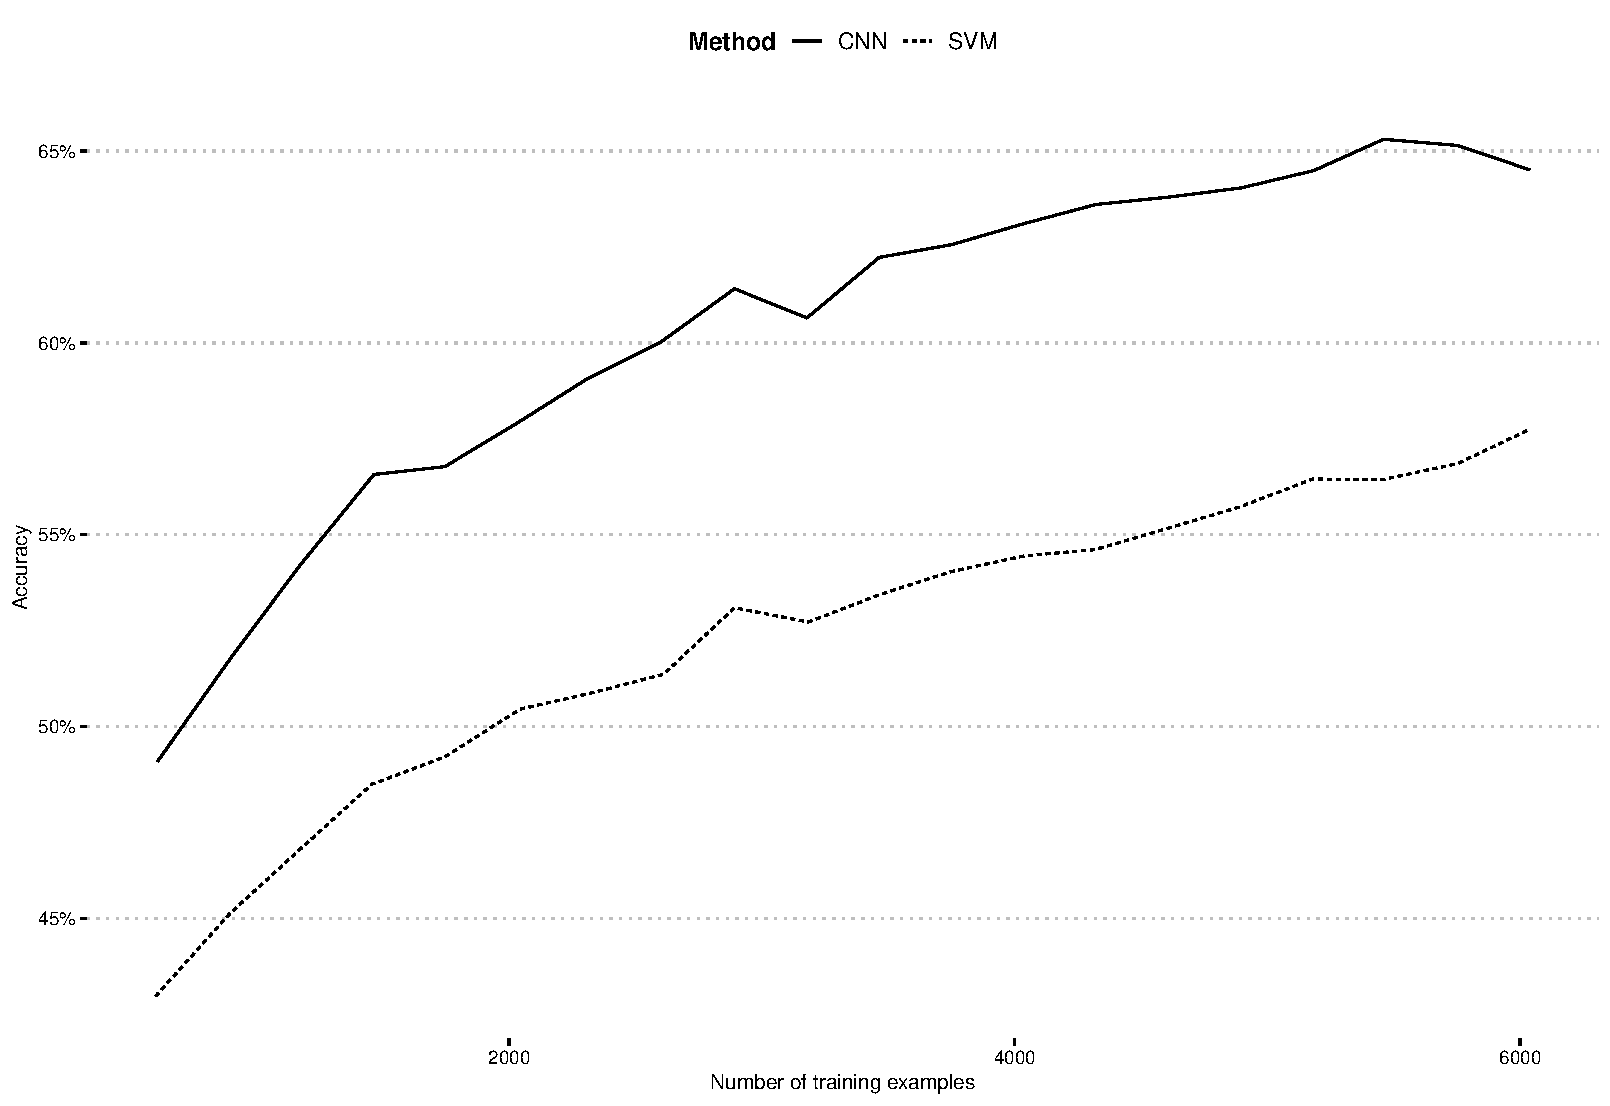
\includegraphics[width=.8\textwidth]{figures/fig_curve.pdf}}

\emph{Note:} Each line shows how quickly more training examples allowed the algorithm to improve performance on the gold standard. For example, with 2000 training documents from the original data of \cite{boukes2019}, the SVM model achieved an accuracy of about 50\%, which increased to almost 55\% with 4000 examples.
\end{figure*}

\noindent Finally, Figure~\ref{fig:curve} shows the so-called `learning curve' of both machine learning algorithms. 
This figure shows the increase of the algorithms' performance as the number of training examples (i.e. more new sentences) increases.
The learning curve was estimated by training on random subsets of the training data and testing against the gold standard,
and gives an indication of how many training documents are needed to achieve a given performance. 
This curve shows that, as expected, both methods improve most quickly at the beginning, signaled by a steep incline, before leveling off to a presumed asymptote, where adding more training examples no longer increases their performance. 
The climbing lines for both algorithms indicate that presumably neither method is saturated yet, assuming the slight downturn at the end of the CNN curve is an anomaly. 
Thus, one can expect that the performance of both methods will profit from more training data.
However, given that both lines are mostly parallel, there is no indication that the performance of the SVM will converge to the performance of the CNN with an equal amount of training data.
%Hence, it seems that CNN is simply the better method for this task. 

%\begin{figure}[t]
%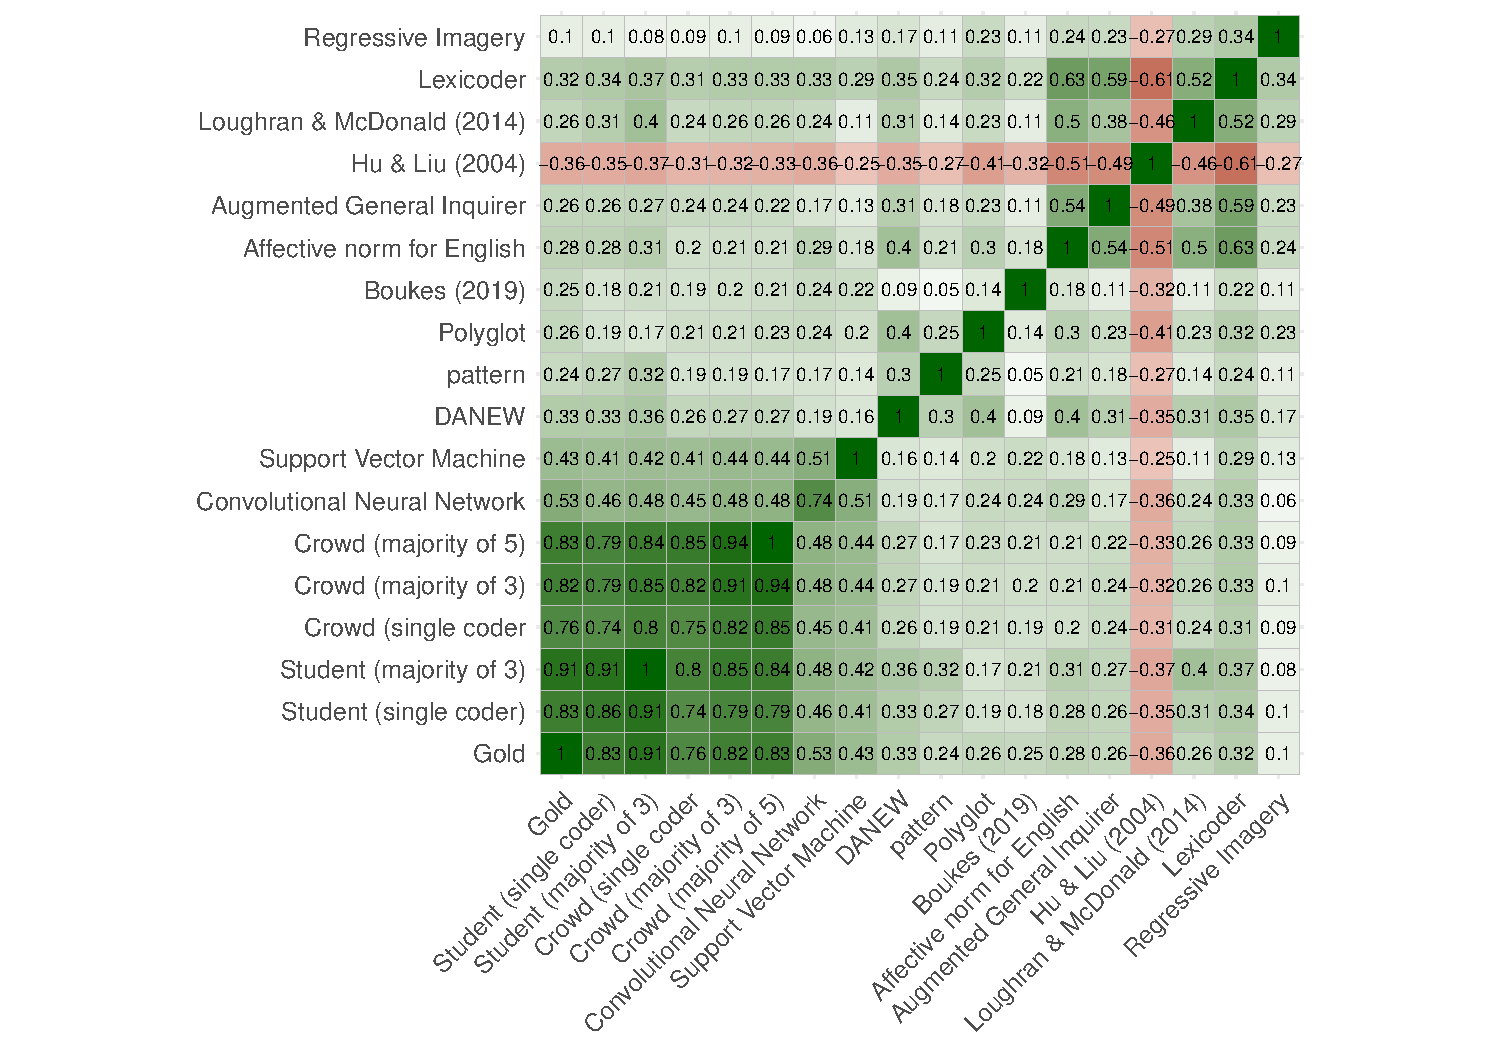
\includegraphics[width=\textwidth]{figures/corr.pdf}
%\caption{Correlation between all methods}\label{fig:corr}
%\textit{Note:} {\small For student and crowd (single coder) and Convolutional Neural Network the average correlation of individual coders/iterations is given. 
%For these methods, diagonal gives the between-coder correlation. }
%\end{figure}

%Figure~\ref{fig:corr} shows the correlation between the various methods. Overall, the methods that correlate weakly with the gold standard also %correlate weakly with each other, showing that there is no systematically different underlying variable that they all measure.
%The only pattern is between the English dictionaries used on the translated headlines, which correlate more strongly with each other than with the gold standard.  

\subsection{Error Analysis}

\newcommand{\fnerroranalysis}{\footnote{%
See `error analysis' in the online appendix at \url{https://github.com/vanatteveldt/ecosent}%
}}

\newcommand{\trans}[2]{\emph{#1} (#2)}

We conducted an error analysis to improve our understanding of the mistakes made by the various automatic methods.\fnerroranalysis{} 
For the error analysis on the off-the-shelf dictionaries, we picked the NRC dictionary, 
the best performing Dutch dictionary (by alpha) that also has an English translation. 
Many of the mistakes made in the Dutch NRC dictionary are missed negations. 
For example positively classifying the word \trans{groei}{growth} in sentences like \trans{afnemende groei hypotheken}{reduced growth in mortgages}  or \trans{matige groei}{tepid growth} or negatively classifying the word \emph{crisis} in \trans{Cyprus heft laatste restricties op na crisis}{Cyprus lifts last restrictions after the crisis}. 
In addition, the error analysis revealed  clear mistakes, such as misclassifying the word \trans{beurs}{stock exchange} as positive. 

The English NRC dictionary applied to headlines translated by deepl shows a similar pattern, with the words \emph{job} and \emph{savings} being misclassified as positive in sentences such as \emph{Best Buy deletes 1500 jobs} and \emph{300 million in savings gone in one day}. The same happened to negative words like \emph{crisis} and \emph{inflation}. 

To better understand the role of translation, we then looked at the sentences that were correctly classified in Dutch but missed by the translated version. An inspection of these ($n=54$) sentences suggests that, although some are translated a bit clumsily, this does not seem to be the cause of the errors as the translation errors are more concerned with function words rather than the sentiment carrying words (for example, \emph{300 million in savings gone in one day} was actually translated as \emph{300 million in savings in one day away}). An interesting detail is that the word \emph{interest} caused most of the translated misclassifications as the English word \emph{interest} is ambiguous between the supposedly neutral meaning of interest rate and the positive concept of being interested or interesting, while the Dutch translation (rente) is not ambiguous. 

For the error analysis of our machine learning approaches, we first look at Naive Bayes as that method has the most interpretable feature weights. Interestingly, the words \trans{faillissement}{bankruptcy} and \trans{werkloosheid}{unemployment} were positive features, presumably because these words are often negated in the training documents. Being based on word frequencies (bag of words), Naive Bayes also suffers from the same lack of context as the dictionaries, for example classifying the sentences \trans{minder woningen onder water}{fewer underwater mortgages} as negative based on negative values for both \emph{fewer} and \emph{underwater}, even though the result of the former is actually to negate the latter. 

The convolutional neural network can take word context into account, but unfortunately the more complex parameters are not easy to inspect manually. When inspecting the misclassified sentences manually, however, it turns out to make some of the same mistakes as the other methods, for example classifying \emph{more bankruptcies} as positive. For many other sentences it is less clear why they are misclassified, although they do seem to have a large amount of rare or new words such as \trans{Werkgevers torpederen caos}{employers torpedo collective-bargaining-agreements}, \trans{dubbelfout bij crisistaks}{double-error with crisis-tax} and \trans{Grieken zijn weer platzak}{Greeks are stone-broke again}. 
Then again, all these words were in the word embeddings and most had sensible synonyms, for example listing \trans{werkgeversheffing}{employer charge} and \trans{graaitax}{grabber tax} as synonyms for \emph{crisistaks}, although \emph{caos} was misclassified 
(presumably due to the failed lemmatization to the singular form \emph{CAO}) and \trans{dubbelfout}{double error} was related mostly to tennis terms. 
Still, since the close synonyms of these rare words are mostly rare words themselves, it is possible that even though the embeddings vectors does words not in the training data to be used for classification, if the words occur in too few contexts in the documents used for creating the embeddings they will still cause difficulties for the algorithm. 






\section{Discussion}

\noindent Determining the tone or valence of statements is an important task for analyzing communication.
Sentiment analysis is not an easy task, however.
Sentiment is conceptually not trivial: statements such as `Libya's Moammar Gadhafi killed', `Brexit was postponed (again)`, or
`House prices skyrocketing' can be positive or negative (or even neutral), depending on your perspective and definition of sentiment. 
Subjective language is also typically more ambiguous and more creative than factual statements,
and even trained expert coders can have serious difficulty agreeing on the sentiment of statements. 

This paper investigated the relatively straightforward (but substantively important) case of differentiating good from bad economic news headlines. %about the economy.
We compared a large number of different methods for measuring this sentiment: 
trained student coders; crowd coding; classical machine learning and deep learning; and a large variety of dictionaries. 
For the latter, we used both original (generic) Dutch dictionaries and generic and domain-specific English dictionaries applied to automatic translation of the text.
The results of all these methods were compared to a gold standard created by coding every unit multiple times and 
resolving any disagreements. 

The main finding is that human coding still carries the day for sentiment coding, 
with only trained students and crowd coding achieving levels of agreement with the gold standard that would generally be accepted as valid measurements. 
Of these, student coding is clearly still better than crowd coding at replicating the gold standard coding,
achieving a Krippendorff's alpha of over 0.9 when using three coders per text.
Crowd coding, however, also has relatively good accuracy, achieving an alpha of over 0.8 when each text is coded multiple times,
equal to the performance of single student coding.
With this performance, crowd coding has a number of substantial advantages over regular student coding. 
First, crowd coding will often be significantly cheaper than student coding. 
For our experiments, we paid coders \$0.02 per sentence. Including test questions, total costs were less than \$50 for 1500 annotations.
This makes it affordable to code all units multiple times, a practice often considered too expensive for manual coding, 
which not only improves the overall point estimate of sentiment, but also gives a measure of spread \citep[cf.][]{benoit16,lind2017content}.
A second advantage is that after setting up the job, almost no researcher effort is required,
as the system takes care of recruiting, testing, and monitoring the coders. 

Please note that this does not mean we endorse the economics or business models of current crowd coding providers. 
In our view, the main benefit of crowd coding is that the process is inherently transparent. 
Since coders are interchangeable and all training and selection happens within the system, 
we can be sure of the exact training and material that the coders received.
With expert (or student) coding, the presumed standard practice is to have training events where groups of coders are instructed
in the codebook and the coding routines. 
Although ideally the training procedure would be published together with the codebook,
it is difficult to avoid coders talking with each other and with the instructors, meaning that it is possible that a shared
understanding can arise that is not captured in the codebook.
This potentially makes it hard to create truly replicable coding and implies that the published intercoder agreement can be overly optimistic. 
For crowd coding, in contrast, there is no reason to assume why the outcome will be structurally different if another researcher launches the same job, guaranteeing replicability and validity of the reliability measure. 
This is in line with the findings and recommendations of \citet{weber18}, who advocate crowd coding after having difficulty replicating their own previous codings of moral claims.

Dictionary coding is probably the most used automatic sentiment analysis method in the social sciences due to its transparency and simplicity.
Unfortunately, but not surprisingly given previous results \citep{boukes2019,soroka15,gonzalez15}, performance of dictionaries was not satisfactory. 
Agreement was generally close to chance agreement, and correlations between dictionaries were also low.
Error analysis showed that this was mostly due to the missing context of words.
This holds for both Dutch dictionaries and for English dictionaries applied to the automatically translated texts.

In line with findings from the computational linguistics community, machine learning significantly outperformed dictionary coding,
with a ``deep learning'' convolutional neural network 
scoring around 20 percentage points higher on both agreement and intercoder reliability measures \citep{rudkowsky2018more,semeval,liu12}. 
This performance is notwithstanding the fact that a relatively low amount of training material was available, 
implying that better results might still be achievable with more training data.
It is also possible that the machine learning models had particular difficulties with the low number of words in each headline,
which could have exacerbated this data scarcity problem. 
This could also explain the higher performance of the CNN model. 
Because this model used word embeddings vectors rather than the word counts (as in the NB and SVM models),
the model could utilize the words in the gold standard headlines even if these words did not occur in the training data.
The disadvantage of machine learning methods are, however, their relative lack of transparency and the need for coded training data.
The fact that a model is based on specific training data also means that a different task or domain requires new training data,
so for smaller tasks it might be better to just use manual coding on a sufficiently large sample. 

\subsection*{Recommendations for Text Classification}
\noindent There are many different techniques for sentiment analysis and classifications of texts more generally. 
Unfortunately, the results of this article show that automatic techniques do not always perform sufficiently.
This even holds for dictionaries that have been developed and validated independently: 
Since tasks and domains are almost never interchangeable in social science, 
validated performance on the task a tool was developed for does not guarantee sufficient performance on a new task.

On the basis of these findings, we recommend that text classification projects should follow the following steps to guarantee validity:

\begin{APAenumerate}
\item Formalize the conceptualization and operationalization for manual annotation of the quantity of interest. 
  This step is extremely important and often requires pilot coding of material and discussion between researchers.
\item Annotate a sufficiently large gold standard for validation. 
  This needs to be coded by at least two annotators to calculate inter-coder reliability (or three in the case of disagreements). The size of the sample depends on the number and distribution of categories, but a good indication is Table 11.2 in \citet[p.240]{krippendorff12} which shows that often between 100 and 300 units are required. If insufficient reliability is achieved, go back to step one and repeat; otherwise, finish the validation set by discussing and resolving all disagreements. 
\item Apply any applicable off-the-shelf dictionaries. 
  If any of these is sufficiently valid as determined by comparison with the gold standard, we recommend using this for the text analysis as dictionaries give very good transparency and replicability for a low cost.
\item If no sufficiently valid off-the-shelf dictionaries exist, consider customizing a dictionary or creating one. 
  In this case, it is paramount that the gold standard is not referenced when creating a dictionary as that would bias the validity estimate: 
  Any person involved in annotating the gold standard cannot contribute to creating the dictionary.
  It can be very beneficial to use corpus statistics of the texts under study, for example by listing the most frequent or surprising words in the corpus or by listing words that are similar to words in an existing dictionary \citep{amsler20}. 
  For example, similar to the results of the error analysis presented above this would have shown that a word like \trans{beurs}{stock exchange} is relatively frequent in this corpus and occurs in the NRC sentiment dictionary, but in the corpus of this study has no clear positive or negative valence and should probably be dropped from the dictionary.
  As always, make sure the corpus analysis excludes any documents in the gold standard to avoid biasing the performance estimate.
  As above, test the validity of the created dictionary against the gold standard, and use it if it is sufficiently valid.
  If many variations need to be tested or threshold scores need to be determined, a second set of documents should be annotated for this. Only the final dictionary should be tested against the validation set to ensure an unbiased estimate of validity. 
\item If off-the-shelf or custom dictionaries do not achieve sufficient validity, the remaining options are human coding or machine learning. 
 For this, code a relatively large set of articles (a thousand or more) using crowd coding or expert coding. 
 We would recommend to use the validation set created in step 2 to continually test the validity of the manual coding by including a small percentage of validation sentences in the jobs. 
\item Train a machine learning model using the coded documents. 
  Use \emph{cross-validation} to perform a first validation and/or test multiple models and select (hyper)parameters as needed. 
  If the model is sufficiently valid, train again using the whole coded data set and validate against the gold standard. 
\item If needed, repeat from step 5 until the model is sufficiently valid or enough units have been coded to perform the substantive analysis. 
\end{APAenumerate}

\vspace{1em}

\noindent Following these guidelines ensures that the results are valid and replicable with the minimum amount of manual coding needed,
which can range from only coding the gold standard to having to do a fully manual analysis. 

We would like to close with a final recommendation for the field. 
In our view, the biggest problem facing the analysis of sentiment or tone in communication science is the lack of a shared conceptualization.
`Sentiment' can mean many things in different theoretical contexts, as is clear from the fact that, for instance, a hotel review, a political policy preference,
and a statement about the economy can all be seen as expressions of sentiment. 
To remedy this situation, we should categorize the different theoretical claims related to tone or sentiment,
and formalize a set of definitions that can be used to create gold standards for each type of sentiment measure.
Specifically, attention should be paid to the unit of measurement and to disentangle the value of the sentiment from its source (who is expressing the sentiment) and target (who or what is being evaluated). 
As a field, we could then collaborate on creating training material and building, comparing, and improving shared tools for one or more 
concrete sentiment analysis tasks as defined in the first step.
This approach of creating \emph{shared tasks} has yielded very good results in computational linguistics and related fields
and have the potential to dramatically increase the quality, comparability, and transparency of automatic sentiment analysis in the social sciences. 

%Voeg toe: i miss one recommendation: Have at least two (or three in the case of disagreements) code a single piece of text to assure the reliability of individual coding decisions.

\newpage
\bibliographystyle{apacite}
{\footnotesize\bibliography{bibliography}}


\end{document}
